% !TEX root = ../main.tex
% chktex-file 21
% chktex-file 46
\section{Effects of Coarsening}%
\label{sec:cons}

We have just seen how to compute a coarsened graph $G_c$ via the REC algorithm.
What remains to be answered now is how coarsening affects the performance of graph algorithms when $G_c$ is used as a proxy for the original graph $G$.
In the first step we will introduce a graph similarity measure.
Using this measure we will then put bounds on the dissimilarity of $G$ and $G_c$.
Finally we will use those bounds to analyze the influence of coarsening on the performance of the \textit{spectral clustering algorithm}.

\subsection{Restricted Spectral Similarity}%
\label{sec:cons:rss}

To compare a graph $G$ with its coarsened version $G_c$ we will use the notion of \textit{spectral similarity}.
As we have seen before, $G$ can be viewed as an operator that transforms an input signal $x \in \mathbb{R}^N$.
We described this transform in terms of the graph's Laplacian $L$,
more specifically in terms of the Laplacian's eigenbasis ${\{ u_k \}}_{1 \leq k \leq N}$ and spectrum ${\{ \lambda_k \}}_{1 \leq k \leq N}$.
Similarly the coarsened graph $G_c$ can be described in terms of its Laplacian $L_c$.
Since $L \in \mathbb{R}^{N \times N}$ and $L_c \in \mathbb{R}^{n \times n}$ act on signal spaces of different dimensionality, they however cannot be compared directly.
Instead we will compare $L$ with $\widetilde{L} = C^{\top} L_c C$, an upsampled version of $L_c$.
We say $\widetilde{L}$ is an \textit{$\epsilon$-approximation} of $L$ iff.\  $\widetilde{L}$ scales all eigenvectors $u_k$ of $L$ by a factor of roughly $\lambda_k$ in the direction of $u_k$:
\begin{wrapfigure}{l}{0.32\textwidth}
	\centering
	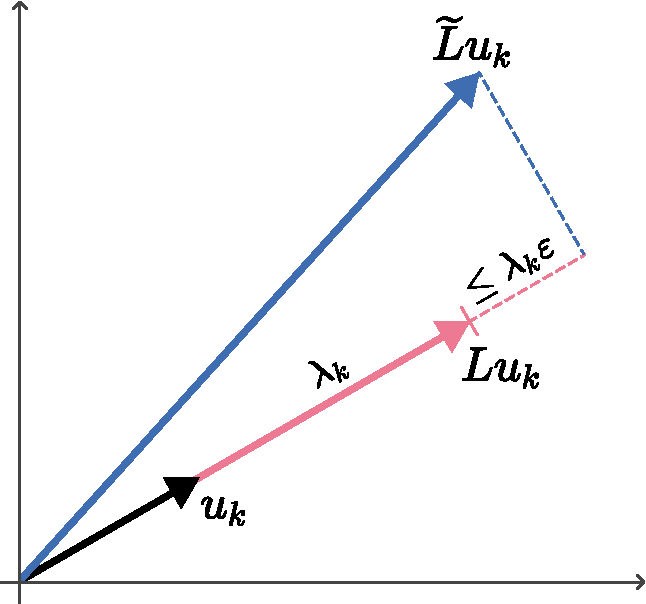
\includegraphics[width=\linewidth]{gfx/cons/rss.pdf}
	\caption{Illustr.\ of \cref{eq:cons:rss}.}\label{fig:cons:rss}
\end{wrapfigure}
\begin{align}
	(1 - \epsilon) \lambda_k \leq u_k^{\top} \widetilde{L} u_k \leq (1 + \epsilon) \lambda_k\quad\text{with } \epsilon \geq 0\label{eq:cons:rss}
\end{align}
For $\epsilon = 0$ this definition implies $L = \widetilde{L}$.
There is however one problem if we require \cref{eq:cons:rss} to hold for \textit{all} eigenvectors $u_k$ of $L$.
The rank of $L$ is $N - 1$, since it has $N$ orthogonal eigenvectors of which $u_1 \in \ker(L)$ does not increase the rank\footnote{%
	More generally $\text{rank}(L) = N - c$ if $G$ has $c$ connected components.
};
similarly $\text{rank}(\widetilde{L}) = n - 1$.
Thus there must be some eigenvector $u_k$ of $L$ with $\lambda_k > 0$ that lies in the null space of $\widetilde{L}$.
For this eigenvector \cref{eq:cons:rss} can never be satisfied, meaning no $\widetilde{L}$ can be an $\epsilon$-approximation of $L$.

\subsection{Putting an RSS-bound on REC}%
\label{sec:cons:bound}

\subsection{Implications for Spectral Clustering}%
\label{sec:cons:sc}
